\section{Zielsetzung}
\label{sec:Zielsetzung}

Ziel des Versuches ist es, die effektive Masse der Leitungselektronen in n-dotiertem Galliumarsenid (n-GaAs)
mit Hilfe des Faraday-Effekts zu bestimmen.

\section{Theorie}
\label{sec:Theorie}

\subsection{Bandstruktur}
\label{sub:Bandstruktur}
Die elektronischen Energiezustände in einem Kristall können durch das Bändermodell beschrieben werden.
Jedes Atom besitzt ein diskretes Energiespektrum. Wenn mehrere Atome angenähert werden und miteinander
wechselwirken überlappen sich diese Spektren. In Kristallen können die Energieniveaus als breite Bänder angenommen werden.
Das Bändermodell besagt, dass jeder Körper ein Valenzband besitzt, dessen Zustände voll mit Elektronen besetzt sind.
Energetisch darüber liegt das Leitungsband, welches freie Zustände für Elektronen besitzt.
Die Besetzung des Leitungsbandes, sowie die Differenz der Energieniveaus der beiden Bänder, die sogenannte Bandlücke,
beeinflussen die Leitfähigkeit eines Materials.
Es werden drei Formen unterschieden:
Im Metall (Leiter) überlappen das Leitungs- und das Valenzband. Die Bandlücke verschwindet somit und das Leitungsband ist mit Elektronen besetzt.
Im Isolator (Nichtleiter) ist die Bandlücke so groß, dass sie von den Elektronen im Valenzband nicht überwunden werden kann. Es gibt somit keine
besetzten Zustände im Leitungsband.
Im Halbleiter ist eine Bandlücke vorhanden, diese kann jedoch, anders als beim Isolator von den Elektronen überwunden werden, wenn diese angeregt werden.
Diese Anregung kann über zugefügte Energie in Form von Wärme entstehen.
Wird keine Energie hinzugefügt, befinden sich die Elektronen im Valenzband in einer festen Bindung und können die Lücke
nicht überwinden, der Stoff ist somit nicht leitend.
Gelangt bei einem Halbleiter ein Elektron in das Leitungsband, entsteht durch das fehlende Elektron ein Loch in dem Valenzband, sodass zwei freie 
Ladungsträger entstehen.
Zusätzlich zur thermischen Anregung können bei Halbleitern durch Dotierung auch gezielt Ladungsträger eingebracht werden.

\subsection{Dotierung}
\label{sub:Dotierung}

Eine Dotierung von Halbleitern mit Fremdatomen erhöht die Anzahl der elektrischen Ladungsträger im Kristall.
Somit kann durch die Dotierung die Leitfähigkeit eines Halbleiters beeinflusst werden.
Man unterscheidet zwischen der p- und der n-Dotierung. Die Auswirkungen der Dotierung sind schematisch in \autoref{Dotierung} dargestellt.
\begin{figure}[H]
    \centering
    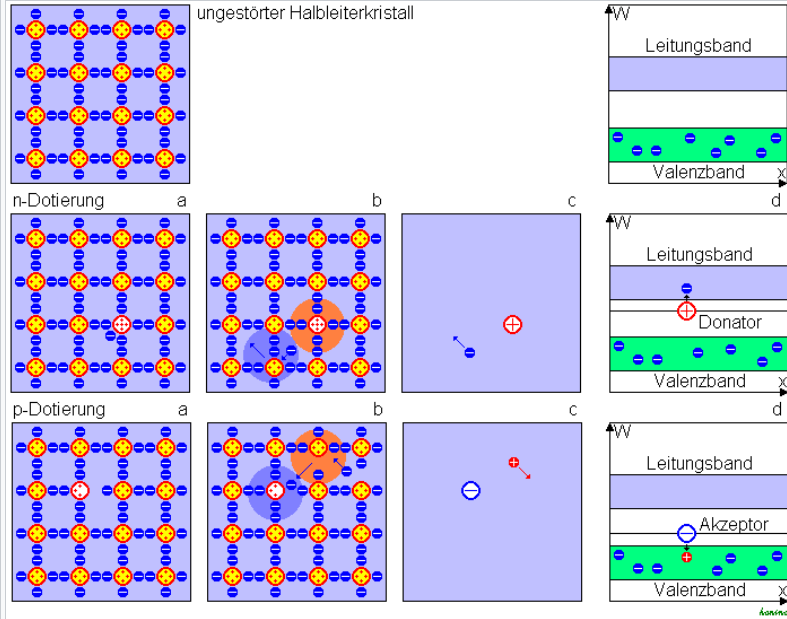
\includegraphics[scale=0.45]{Abbildungen/Dotierung.png}
    \caption{Schematische Skizze zur Dotierung von Halbleitern.\cite{Dotierung}}
    \label{fig:Dotierung}
\end{figure}
Bei der p-Dotierung wird ein Akzeptor, also ein Atom mit weniger Valenzelektronen als der Halbleiter, in den Kristall eingebracht.
Der Akzeptor erhöht das Valenzband, und durch das fehlende Valenzelektron entsteht eine ortsfeste negative Ladung und ein frei bewegliches
positives Defektelektron beziehungsweise Loch.
Die n-Dotierung ist das Gegenteil. Hier wird ein Donator, also ein Atom mit mehr Valenzelektronen als der Halbleiter, in den Kristall eingebracht.
Dadurch entsteht eine ortsfeste positive Ladung und das überschüssige Elektron gelangt ins Leitungsband und wird somit zu einer frei beweglichen
negativen Ladung im Kristall. Das Leitungsband wird bei der n-Dotierung gesenkt.
Bei der Dotierung ändert sich zudem das Gitterpotential an den betroffenen Stellen und die Isotropie des Kristalls geht verloren.
Im Versuch werden n-dotierte Galliumarsenidproben untersucht.



\subsection{Die effektive Masse}
\label{sub:effektiv}
Um die Bewegung von Elektronen in einem Festkörper beschreiben zu können, wird das Konzept der effektiven Masse eingeführt.
Elektronen in einem Festkörper bewegen sich quasifrei. Wird ihre Masse durch eine effektive Masse ersetzt, die den Einfluss des
periodischen Potentials des Gitters auf die Bewegung und kinetische Energie der Elektronen berücksichtigt, können sie als freie
Teilchen betrachtet werden.
Die Betrachtung des Leitungsbandes um das Minimum eignet sich in Halbleitern als Approximation der komplexen mathematischen Bandstruktur.
(siehe \autoref{fig:Band})
\begin{figure}[H]
    \centering
    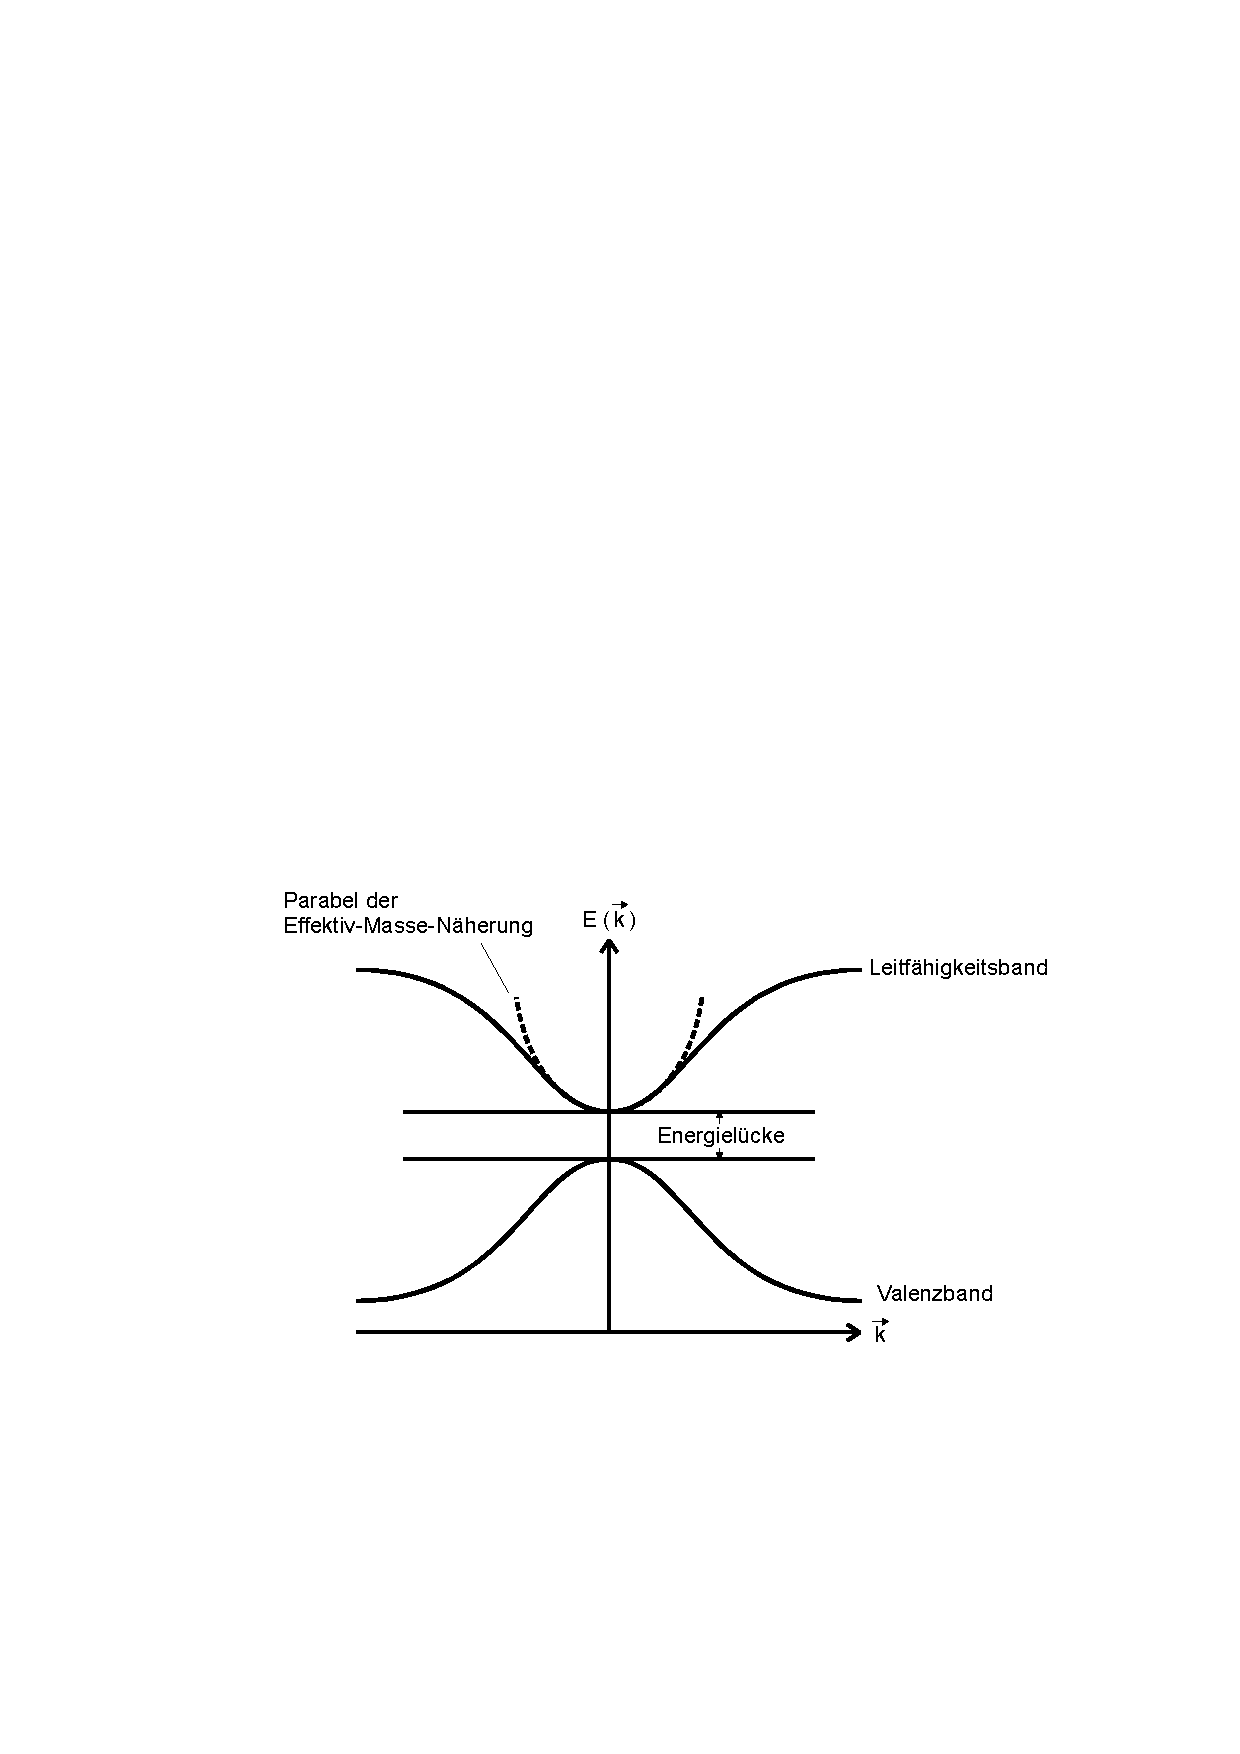
\includegraphics[scale=0.7]{Abbildungen/band.png}
    \caption{Approximation der Bandstruktur im Halbleiter.\cite{Demtröder3}}
    \label{fig:Band}
\end{figure}

Um die effektive Masse herzuleiten wird die Elektronenenergie am Minimum $\varepsilon(\vec{k})$ in eine Taylorreihe um $k=0$ entwickelt
\begin{align*}
    \varepsilon(\vec{k})=\varepsilon(0) + \frac{1}{2}\sum_{i=1}^3 \left. \frac{\partial^2 \varepsilon}{\partial k_i^2}\right|_{k=0}k_i^2 + \mathcal{O}(k^3)
\end{align*}
und mit der Elektronenenergie des harmonischen Oszillators
\begin{align*}
    \varepsilon &= \frac{\hbar k^2}{2m}
\end{align*}
verglichen.
Die effektive Masse ergibt sich somit zu
\begin{equation*}
    (m^*)_{ij} = \hbar^2 \left( \frac{\partial^2 E(\vec{k})}{\partial k_i \partial k_j} \right)^{-1}. 
\end{equation*}


\subsection{Zirkulare Doppelbrechung}
\label{sub:Doppelbrechung}
Zirkuläre Doppelbrechung ist die Fähigkeit eines Kristalls, die Polarisationsebene eines linear polarisierten Lichtstrahls bei der Transmission
zu drehen. Ein Kristall mit dieser Fähigkeit wird optisch anisotrop oder optisch aktiv genannt.

Bei einem optisch aktiven Medium unterscheiden sich aufgrund der Materialstruktur die Phasengeschwindigkeiten für rechts- und linkszirkular
polarisiertes Licht.
Jede linear polarisierte Welle kann gemäß
\begin{equation}
    \vec{E}(z)=\frac{1}{2}(\vec{E_R}(z)+\vec{E_L}(z))
    \label{eqn:E}   
\end{equation}
als Überlagerung zweier entgegengesetzt, zirkular polarisierten Wellen mit gleicher Frequenz dargestellt werden. Dabei gilt
\begin{equation*}
    \vec{E_{L/R}}=(E_0\vec{x}_0\pm \text{i}E_0\vec{y})\exp{(\text{i}k_{L/R}z)},
\end{equation*}
sodass die Polarisation der Welle beim Eintritt in den Kristall parallel zur $\vec{x}$-Richtung liegt.

Mit den Definitionen der Phase
\begin{align*}
    \Psi  &\coloneqq \frac{L}{2}(k_R+k_L)\\
    \shortintertext{und des Winkels}
    \theta&\coloneqq \frac{L}{2}(k_R-k_L)
\end{align*}
ergibt sich nach \autoref{eqn:E} ein Ausdruck des aus dem Kristall der Länge $z=L$ austretenden Lichts zu 
\begin{equation*}
    \vec{E}(L)=E_0 \exp(\text{i}\Psi)\left(\cos(\vartheta) \vec{x}_0 + \sin(\vartheta)\vec{y}_0\right).
\end{equation*}


Die Polarisationsebene wurde demnach um den Winkel $\theta$ bezüglich der Ausgangslage $\vec{x}_0$ verdreht. Durch
Berücksichtigung von $k=\frac{n \omega}{c}$ mit dem Brechungsindex $n$ und der Kreisfrequenz der Welle $\omega$,
kann $\theta$ auch durch 
\begin{equation*}
    \theta=\frac{L\omega}{2c}(n_R-n_L)
\end{equation*}
ausgedrückt werden. Die Drehung der Polarisationsebene um den Winkel $\theta$ ist in \autoref{fig:Doppelbrechung} dargestellt.

\begin{figure}[H]
    \centering
    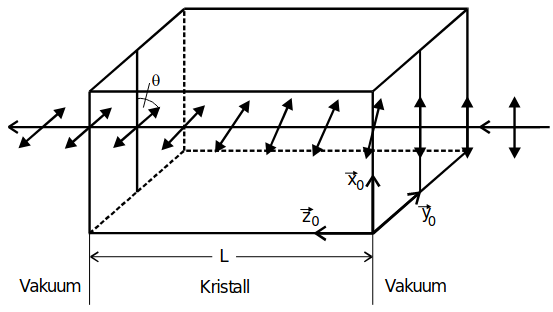
\includegraphics[scale=0.7]{Abbildungen/Doppelbrechung.png}
    \caption{Schematische Darstellung der zirkulären Doppelbrechung.\cite{V46_Anhang}}
    \label{fig:Doppelbrechung}
\end{figure}

Mikroskopisch lässt sich die zirkulare Doppelbrechung durch elektrische Dipole beschreiben, die in dem Material durch das 
Magentfeld induziert werden. Die durch die Dipole erzeugte Polarisation des Kristalls 
\begin{equation*}
    \vec{P}=\varepsilon_0\chi\vec{E}
\end{equation*}
ist abhängig von der dielektrischen Suszeptibilität des Stoffes. Hierbei ist $\varepsilon_0$ die Influenzkonstante und $\chi$ die
dielektrische Suszeptibilität, welche in anisotropen Kristallen als Tensor $\overline{\chi}$ geschrieben wird.
Ein Material ist doppelbrechend, wenn
\begin{equation}
    \overline{\chi}=
    \left[
        \begin{array}{ccc}
        \chi_{xx}          & +i\chi_{xy} & 0         \\ 
        -i\chi_{xy}   & \chi_{yy}        & 0         \\
        0                  & 0                & \chi_{zz}
    \end{array}
    \right]
    \label{eqn:chi}
\end{equation}
gilt.
Wenn die Suszeptibilität jedoch keine komplexen Matrixeinträge aufweist, so tritt keine Doppelbrechung auf.
Ein solches Material wird als optisch isotrop beziehungsweise optisch inaktiv bezeichnet. 


\subsection{Der Faraday-Effekt für optisch inaktive Materie}
\label{sub:Faraday}
Durch Anlegen eines Magnetfeldes kann auch ein optisch isotropes Material doppelbrechend werden.
Dieses Phänomen wird Faraday-Effekt genannt.
durch die Betrachtung
Die gebundenen Elektronen in der Probe, welche zusätzlich durch ein magnetisches
Feld gestört werden, können durch die Bewegungsgleichung
\begin{align}
    m\ddot{\vec{r}}+K\vec{r}&=-\text{e}_0\vec{E}(\vec{r})-\text{e}_0\dot{\vec{r}}\times\vec{B}
    \label{eqn:klassische_Bewegungsgleichung}
\end{align}
beschrieben werden.
Die Auslenkung des Elektrons aus der Gleichgewichtslage wird hierbei durch $\vec{r}$ beschrieben, die
Konstante K bezeichnet die Bindung des Elektrons an seine Umgebung und die Elementarladung ist gegeben durch e0.
$\vec{E}$ stellt die Feldstärke der einfallenden Lichtwelle dar.

Der Ausdruck für den Drehwinkel der Polarisationsebene $\theta$ 
\begin{align}
   \frac{\theta}{L}& \approx \frac{\text{e}_0^3\lambda^2 NB}{8\pi^2\varepsilon_0\text{c}_0^3}\frac{1}{m^2 \cdot n} = \frac{\text{e}_0^3\lambda^2 NB}{8\pi^2\varepsilon_0\text{c}_0^3}\frac{1}{m^{*2} \cdot n}\\
    \label{eqn:drehwinkel}
\end{align}
kann aus \autoref{eqn:klassische_Bewegungsgleichung} hergeleitet werden.\\
Die Länge $L$ enstpricht der Dicke der Probe, $B$ bezeichnet die Magnetfeldstärke am Ort der Probe, $\lambda$ ist die Wellenlänge des
Interferenzfilters und $N$ die Dotierung der Probe. Durch $n$ wird der Brechungsindex gegeben.\\
Nach \autoref{sub:effektiv} darf $m$ in der Gleichung durch $m^*$ ersetzt werden.